%=====================================================================
\section{Block size and purity}\label{sec:purity}

Each chain resizes itself from the fee rates its payers choose. \emph{Purity} is the fees paid divided by the value transacted over a day of payments (96, 288 or 576 blocks), so each payment counts by its size and the target is the standard fee, 1\% on Jen \st{Decided, revised October 2026}. An earlier rule took the geometric mean of fee rates counted per payment; a flood of tiny payments at the top rate could move it for almost nothing, and minters now also rank payments by fee, not by fee rate (Section~\ref{sec:accounts}). It answers one question: are payers paying for speed?

\begin{itemize}
\item \textbf{Grow} when the recent fee rate is above 1.02\% on Jen and blocks average over 90\% full, each block's fullness counted against what the cap allows for the time the block took (at least a quarter of the target time) \st{Decided, Jen-0.11}.
\item \textbf{Hold} when fees are high but blocks are not full: the problem is too few provers, not too little room.
\item \textbf{Shrink} only when fees are at the standard rate and blocks are under 60\% full.
\end{itemize}

Steps on Jen are $+0.3\%$ per block to grow and $-0.12\%$ to shrink. Hard ceilings are 4\,MB (Yen), 3\,MB (Ken) and 2\,MB (Jen); until nodes check one proof per block, the 1,024-leaf verification limit is lower. Faking congestion costs money: half of each fee goes into a pool that pays $1/32$ of itself to each later block, so fees paid to oneself are partly lost. On the Jen-0.7 devnet, capacity per blow rose from 4 to 16 payments when 70\% of payments chose fineness 940 and fell back to 4 when 60\% chose 9999.

\paragraph{No cross-chain consensus dependency.} A joint resize of the three chains was considered and dropped: Jen, the cheapest chain to fill with fake fees, could then resize Yen, and a stall on Jen would spread. Demand that Yen cannot hold instead flows down to Ken and Jen through higher Yen fees, and wallets route payments through the cheaper metals \st{Decided}.

%=====================================================================
\FloatBarrier
\section{The coin weight: one \JEN{} is one \SEN}\label{sec:peg}

This section is the heart of Zen. Balances, fees and rewards are counted in fixed base units (pico). A coin weighs $S$ base units, and $S$ is what the network reads the physical coin to be worth, so $1~\JEN = 1~\SEN$ by definition of $S$; each chain has its own $S$. The section explains how $S$ is read, how the reading is defended, what an attack costs, and how fast $S$ reaches the truth.

\subsection{Fee limits in coins}\label{sec:w}
The fee limits are set in coins, so they follow $S$ \st{Decided, revised October 2026}. The smallest fee is 0.01 coin, and the smallest payment is the smallest fee divided by the chain's top fee rate, so the smallest payment at the top rate pays exactly the smallest fee:

\begin{center}\small
\begin{tabular}{l r r r}
\toprule
 & \textbf{Golden Yen} & \textbf{Silver Ken} & \textbf{Bronze Jen}\\
\midrule
Fee limits & 0.01\%--2.5\% & 0.01\%--4.5\% & 0.01\%--6\%\\
Smallest fee & 0.01~\YEN & 0.01~\KEN & 0.01~\JEN\\
Smallest payment & 0.4~\YEN & $\tfrac29$~\KEN & $\tfrac16$~\JEN\\
\bottomrule
\end{tabular}
\end{center}

With a Sen at \$0.0276, the smallest Jen payment is about \$0.005 and the smallest fee about \$0.0003. The resize (Section~\ref{sec:purity}) keeps the price of block space near the standard fee, so a payment costs about its standard rate of what it moves, however the chain is used.

An earlier draft set these limits from $W$, the typical payment size. A floor tied to payment sizes rises when large payments dominate: a typical payment of 600,000~\JEN{} would make the smallest payment 1,000~\JEN, about \$27, and lock small payers out just as the chain became popular. $W$ also had its own attack (a fifth of all payments for a week moved it by up to 50\% in simulation). Setting the limits in coins removes both. The cost is that the limits follow $S$, so an attack on the peg moves them too, but only within $S$'s band: at worst from $\tfrac16$ to about $\tfrac19$ or $\tfrac14$ Sen. Before the peg converges, the floor floats with whatever a Jen is worth, and the launch rules may start lower.

\subsection{Reading $S$ from coin-priced payments}
Payments come in two modes, told apart by the amount alone \st{Decided in principle}:
\begin{itemize}
\item \textbf{Coin-priced} (``Sen-priced''): a shop prices in coins. The amount is an exact whole number of sixths of the $S$ of one of the last 8 blocks, so the network reads the price in Sen. A converted amount essentially never lands on an exact sixth by chance: none of 200,000 random amounts did in the Jen-0.9 test.
\item \textbf{Ordinary}: any other amount, for example converted from another currency. The network reads its value in base units.
\end{itemize}

The two modes describe the same goods. If the typical coin-priced basket costs $p$ Sen and the typical ordinary payment is worth $v$ base units, a Sen is worth about $v/p$ base units, and that is where $S$ moves:
\begin{equation}
S_{\text{target}} = \frac{\text{typical ordinary value (base units)}}{\text{typical coin-priced price (in coins)}} .
\end{equation}
The physical metal enters at exactly one point: shops that set their coin prices from what the physical coin buys. A shop that converts from the network's own rate merely reports $S$ back to itself (Section~\ref{sec:converge}).

\begin{figure}[tbp]
\centering
\begin{tikzpicture}[node distance=4mm and 5mm,
  st/.style={box,minimum height=1.25cm,text width=2.25cm,font=\sffamily\scriptsize}]
  \node[st,fill=copperwash] (pay) {\textbf{Payments}\\ coin-priced (exact sixths) and ordinary};
  \node[st,right=of pay] (once) {\textbf{Each gram once}\\ rested $-$ used; 3-day rest};
  \node[st,right=of once] (cd) {\textbf{Coin-days}\\ value $\times\min(\text{age},30)/30$};
  \node[st,right=of cd] (rcv) {\textbf{Receivers}\\ 0.03\% cap, 7-day bond, penalty};
  \node[st,right=of rcv] (mid) {\textbf{Day reading}\\ middle 20\% of counted value};
  \node[st,below=9mm of mid,fill=bluewash] (med) {\textbf{Median of three}\\ payments, two exchange pairs};
  \node[st,left=of med] (win) {\textbf{Day window}\\ Fibonacci over days; 10\% day clip};
  \node[st,left=of win] (frz) {\textbf{Freeze}\\ disagreement day does not count};
  \node[st,left=of frz] (anc) {\textbf{Anchor and band}\\ 2.9\%/day; $\pm10\%$};
  \node[st,left=of anc,fill=wash,line width=1pt] (S) {\textbf{Coin weight $S$}\\ 1 \JEN{} = $S$ base units};
  \draw[arr] (pay) -- (once); \draw[arr] (once) -- (cd); \draw[arr] (cd) -- (rcv); \draw[arr] (rcv) -- (mid);
  \draw[arr] (mid) -- (med); \draw[arr] (med) -- (win); \draw[arr] (win) -- (frz); \draw[arr] (frz) -- (anc); \draw[arr] (anc) -- (S);
\end{tikzpicture}
\caption{How a chain reads its coin weight. Each stage removes one way to fake the reading. The exchange stage applies once Ken and Yen exist; until then Jen relies on its own payments.}
\label{fig:reading}
\end{figure}

\subsection{The defences}\label{sec:defences}
A naive reading is cheap to move. In the Jen-0.11 devnet, one node sending fake coin-priced payments to its own users dragged 1~\JEN{} from 1.0 to 0.31~Sen in 40 blocks. The defences below, simulated in the market model of Appendix~\ref{app:sims}, each remove one way to fake the reading (Figure~\ref{fig:reading}) \st{Proposed, simulated}.

\paragraph{Each gram counts once.} Every account carries three numbers: \emph{rested} (money unmoved for the rest period, 3 days proposed), \emph{fresh} (money received since, with its arrival day) and \emph{used} (rested money already counted this period). A payment counts toward $S$ only up to rested minus used. The payment itself always goes through. The numbers change only when the account sends or receives, and the leaf proof checks them together with the balance, so nothing private is revealed. Money paid around in a loop counts once per rest period. The rules are exact: before a send or receive the account is settled at the block's day (fresh money older than the rest period becomes rested; the used number restarts in a new 3-day period); a payment spends fresh money first, counts the smaller of its amount and rested minus used, and rested money that leaves is the used money first; a receipt adds fresh money and restarts the clock of all fresh money in the account, which is conservative. The account leaf holds five more numbers (11 field elements) and the state leaf proves every transition; a builder that claimed more rested money than the leaf holds produced no proof, and a node replaying the block counts the same amounts as the builder (measured; block data is unchanged, 2,401 bytes for the test block, and the state leaf stays at $2^{13}$ rows, 2.6\,s) \st{Proposed, measured}.

\paragraph{Value weighting.} Because money counts once, the reading weighs payments by value: each day it takes the middle 20\% of counted value, by log price on the coin-priced side and by log value on the ordinary side. Each block adds its counted payments to two fixed histograms of about 1,000 bins; at the end of the day one number per side is kept. Tiny fake payments weigh almost nothing.

\paragraph{Coin-days.} A counted payment weighs its value times $\min(\text{age},30)/30$, where age is how many days its money rested, as in Peercoin's coin age \cite{peercoin}. Honest customers mostly spend money held for weeks and count close to fully. An attacker who cycles money counts at most $C/30$ a day for $C$ dollars, whatever his cycle.

\paragraph{Day window, clip, anchor and band.} The day readings enter a window with Fibonacci weights over days (Figure~\ref{fig:window}). A day's reading may differ from the window before it by at most 10\%. A slow \emph{anchor} follows $S$ by at most 0.005\% a block (2.9\% a day), and $S$ must stay within $\pm10\%$ of the anchor. This is the one hard limit: whatever an attacker spends, $S$ moves at most about 13\% in a week and 37\% in a month.

\begin{figure}[htbp]
\centering
\begin{minipage}[t]{0.42\textwidth}\centering
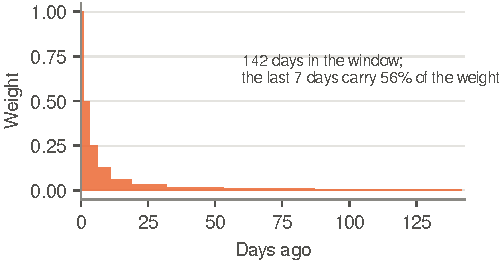
\includegraphics[width=\textwidth]{figs/window.pdf}
\caption{Fibonacci day weights: 1 for the last day, $\tfrac12$ for the two before, $\tfrac14$ for the next three, and so on.}
\label{fig:window}
\end{minipage}\hfill
\begin{minipage}[t]{0.54\textwidth}\centering
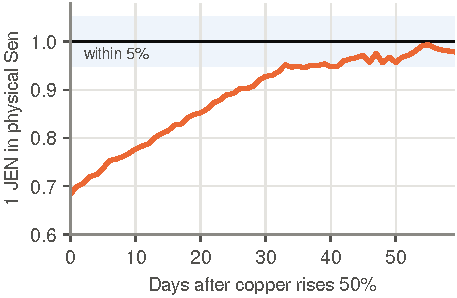
\includegraphics[width=\textwidth]{figs/copper.pdf}
\caption{A genuine change: copper rises 50\% and the network follows. With window, clip, anchor and band, 1~\JEN{} is back within 5\% of 1~\SEN{} in about 39 days (simulated).}
\label{fig:copper}
\end{minipage}
\end{figure}

\paragraph{Receiver cap and bond.} A receiving account counts for at most 0.03\% of the day's counted coin-priced value. It counts at all only if it has held a bond for 7 days (base about \$1,000, set as a share of traffic). Each bonded receiver has one vote, its own price change against its own past. When the value-weighted change differs from the median vote by more than 3\%, the bond required grows 20\% a day, up to 20 times; otherwise it shrinks 5\% a day back to the base. A genuine price move shifts all shops alike and does not raise the bond.

\paragraph{Bond penalty.} Each bonded receiver's 30-day price change is compared with the median receiver's. A receiver more than 15\% away loses 2\% of its bond a day, burned. In simulation 0.1\% of honest shops were ever hit. An attacker must pay the penalty or keep his payments within 15\% of the typical price, which needs far more money for the same push.

\paragraph{Freeze on disagreement.} When receivers disagree beyond the trigger, the day does not count and $S$ holds \st{Proposed}. An alternative, reading the day from the median receiver vote, was rejected: an attacker with many bonded accounts (about 2,600 for \$25M) outvotes the 730 honest ones and reached a 39\% move.

\paragraph{Standard fee and settlement.} Only payments paying at least the chain's standard fee count (1\% Jen, 0.4\% Ken, 0.1\% Yen). Nothing in the protocol converts value automatically at $S$: contracts, loans and salaries that refer to $S$ use its 30-day average, so a short push gains little, and $S$'s lag behind genuine moves cannot be exploited the way Iron Finance's lagging price was \cite{ironfinance}.

\subsection{What the defences do}
Figure~\ref{fig:daywin} shows a month-long attack by a participant making 10\% of all payments, all of them fake coin-priced payments at the price that pushes hardest. With the day window alone, 1~\JEN{} falls to about 0.45~\SEN{} and recovers only after the attack ends. The anchor and band alone do not help much against this push, because the window has already moved before the band binds. With the day clip as well, 1~\JEN{} falls only to about 0.75~\SEN{} by day 30, at the anchor's pace, and the network recovers within weeks.

\begin{figure}[htbp]
\centering
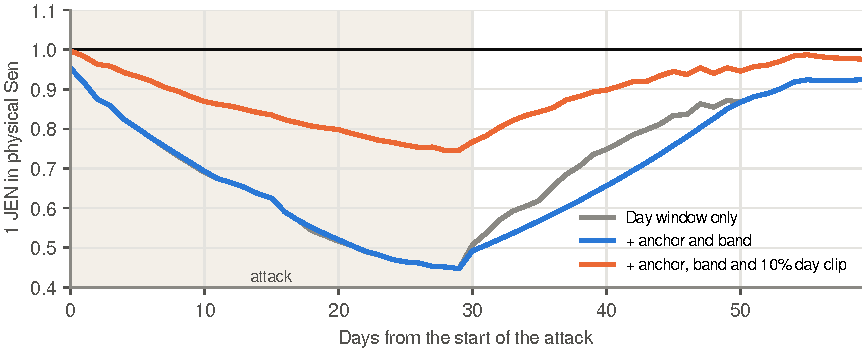
\includegraphics[width=0.92\textwidth]{figs/daywin.pdf}
\caption{A 30-day attack by 10\% of all payments, under three versions of the reading (simulated, \texttt{daywin.js}). The shaded band is the attack.}
\label{fig:daywin}
\end{figure}

Table~\ref{tab:defences} and Figure~\ref{fig:coindays} give the attacker's cost on Jen at one million payments a day, \$2.47M of coin-priced value a day. Normal wander of $S$ is 2--4\%.

\begin{table}[htbp]
\centering\small
\begin{tabularx}{\textwidth}{Y l r r r}
\toprule
\textbf{Defences} & \textbf{Attacker's money} & \textbf{Move 7 d / 30 d} & \textbf{Locked} & \textbf{Lost in 30 d}\\
\midrule
Day window, count-weighted, fees only & fees & 13\% / 31\% & -- & \$3k / \$10k\\
Full set (each gram once, value weighting, cap, bond) & \$1M & 13\% / 16\% & \$2.2M & \$27k\\
Full set & \$5M & 11\% / 20\% & \$11M & \$177k\\
+ coin-days & \$1M & 6\% / 6\% & \$1.2M & \$10k\\
+ coin-days & \$5M & 13\% / 19\% & \$6.4M & \$42k\\
+ bond penalty & \$1M & 12\% / 17\% & \$2.3M & \$417k\\
+ coin-days + bond penalty & \$1M & 4\% / 6\% & \$1.2M & \$116k\\
+ coin-days + bond penalty & \$5M & 12\% / 18\% & \$6.2M & \$534k\\
+ coin-days + bond penalty & \$25M & 13\% / 23\% & \$30M & \$2.7M\\
\bottomrule
\end{tabularx}
\caption{Largest move of $S$ for the attacker's best strategy, money locked (attacker's money and bonds) and money lost in 30 days (fees, 5\% a year interest and burned penalties). Jen at one million payments a day (simulated, \texttt{volsim2.js}, specification 6.6).}
\label{tab:defences}
\end{table}

\begin{figure}[htbp]
\centering
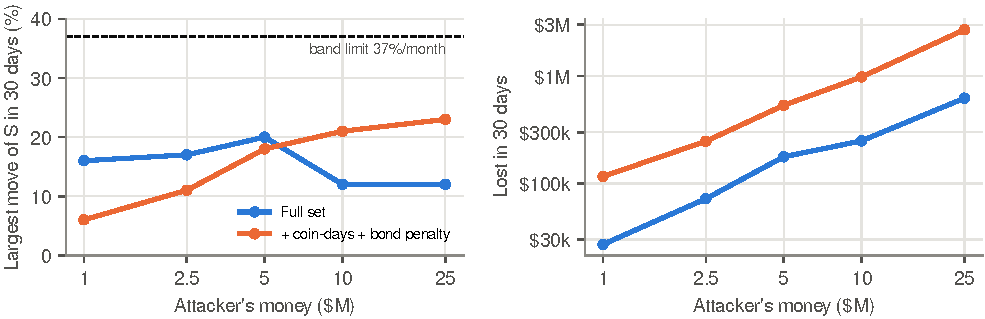
\includegraphics[width=\textwidth]{figs/coindays.pdf}
\caption{Left: the largest 30-day move of $S$ against the attacker's money. Right: what the attack costs him in 30 days. Coin-days and the bond penalty cut what small attackers achieve and multiply what every attacker loses (simulated, \texttt{volsim2.js}).}
\label{fig:coindays}
\end{figure}

\subsection{Watchers and defenders}
The disagreement signal is public, so anyone can run a \emph{watcher}: it shows when the reading leaves the median receiver, in which direction, and which new bonded accounts move together. Watchers decide nothing on the chain; they warn wallets (``peg under pressure: settle at the 30-day average'') and let \emph{defenders} act. A defender (shops, exchanges, a community fund) adds real payments at the honest typical price from rested money. Its payments agree with the median, so it pays no penalty and cannot push $S$ past the truth. Half the attacker's money is enough, because the defender strengthens the honest middle that the reading already favours (Figure~\ref{fig:defender}, Table~\ref{tab:defender}).

\begin{figure}[htbp]
\centering
\begin{minipage}[c]{0.5\textwidth}\centering
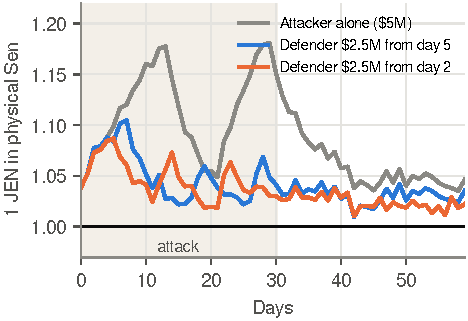
\includegraphics[width=\textwidth]{figs/defender.pdf}
\end{minipage}\hfill
\begin{minipage}[c]{0.47\textwidth}
\caption{A \$5M attacker with all defences, alone and against a defender with half his money joining after 2 or 5 days (simulated, \texttt{defend.js}). The defender brings $S$ back under 5\% within days, at about a twentieth of the attacker's cost.}
\label{fig:defender}
\end{minipage}
\end{figure}

\begin{table}[htbp]
\centering\small
\begin{tabular}{l l l r r r r}
\toprule
\textbf{Attacker} & \textbf{Defender} & \textbf{Joins} & \textbf{Peak} & \textbf{Under 5\% by} & \textbf{Defender spends} & \textbf{Attacker spends}\\
\midrule
\$5M (alone 18\%) & \$2.5M & day 2 & 9\% & day 8 & \$24k & \$534k\\
\$5M & \$2.5M & day 5 & 10\% & day 11 & \$21k & \$534k\\
\$5M & \$5M & day 2 & 6\% & day 7 & \$48k & \$534k\\
\$25M (alone 23\%) & \$12.5M & day 2 & 8\% & day 4 & \$119k & \$2.7M\\
\$25M & \$12.5M & day 5 & 11\% & day 10 & \$106k & \$2.7M\\
\bottomrule
\end{tabular}
\caption{Attacker against defender over 30 days (simulated, \texttt{defend.js}).}
\label{tab:defender}
\end{table}

\subsection{The exchange as a second and third reading}\label{sec:exreading}
Once Ken and Yen exist, every trade between the chains is also a payment on each chain. Some traders quote in coins (``1 \KEN{} for 212 \JEN'', from the metal prices). These coin-priced trades are the exchange's version of coin-priced shop payments. From the day's batch auctions, each chain gets two more readings of its weight:
\begin{equation}
S_{\text{Jen}}^{(\text{Jen--Ken})} = S_{\text{Ken}} \times \frac{\text{Ken grams per Jen gram}}{\text{Jen coins per Ken coin}},
\end{equation}
and likewise from Jen--Yen. The day's value for each chain is the \textbf{median of three}: its own payments and the two exchange readings \st{Proposed, simulated}. An attacker must win two of the three. Exchange readings are hard to fake: the order book is open and every trade in a batch clears at one price, so an order at a wrong coin ratio is filled by others, who profit from it.

\begin{figure}[htbp]
\centering
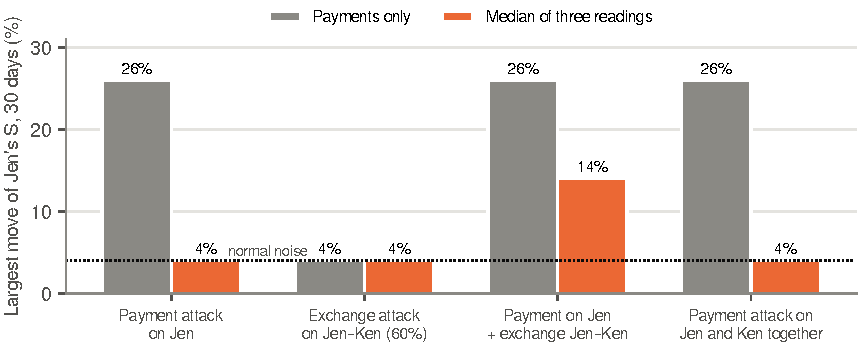
\includegraphics[width=0.92\textwidth]{figs/exchange.pdf}
\caption{Largest 30-day move of Jen's $S$ with and without the exchange readings (simulated, \texttt{tri2.js}). A payment attack on one or two chains is held to normal noise; moving Jen requires also holding the exchange.}
\label{fig:exchange}
\end{figure}

With \$5M a day of coin-priced Jen--Ken trading, holding 60\% of it at 13\% off the true ratio loses the attacker about \$1M a day to the traders who fill him: about \$30M a month for a 14\% move (Figure~\ref{fig:exchange}). The same comparison doubles as a \textbf{counterfeit detector}: when one chain's payment reading departs from both of its exchange readings while the other chains stay normal, trust in that chain's physical coin has changed, for example through counterfeit Ren. The median keeps the electronic coin at its metal value meanwhile, and the community checks the physical coins (weight, size, conductivity, assay).

\subsection{What an attack costs}
Figure~\ref{fig:costs} summarizes the layers. A 12\% push held for a month on Jen at one million payments a day costs about \$3k in fees with no defences; about \$45k a month and \$1.9M locked with each gram once, the cap and the bond; about \$0.5M a month and \$6M locked with coin-days and the penalty; and about \$30M a month once Ken and Yen trade. The simulations assume the attacker already holds the coins. He cannot print them: he must mine or mint them, buy them (raising their price, and holders of money that keeps its value are reluctant to sell it for weaker money, Thiers' law), turn metal into them, or borrow them, and borrowed coins arrive fresh with no coin-days. Every defence is paid in Zen, so security grows with adoption, as Bitcoin's hash rate makes a 51\% attack harder as it grows. The weakest period is the start, when the largest holders are the first miners and minters, who also have the most to lose if the peg breaks.

\begin{figure}[htbp]
\centering
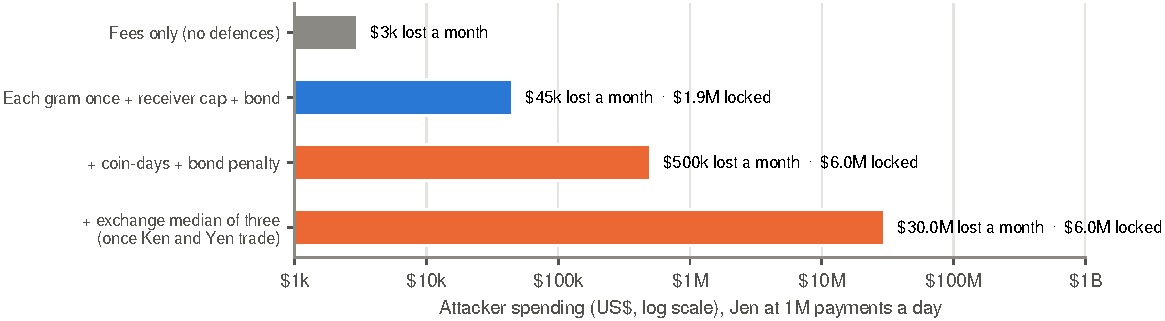
\includegraphics[width=\textwidth]{figs/costs.pdf}
\caption{Cost of holding a 12\% push on Jen's $S$ for a month, by defence level (simulated; log scale). Each layer multiplies the cost roughly tenfold.}
\label{fig:costs}
\end{figure}

\begin{table}[htbp]
\centering\small
\begin{tabularx}{\textwidth}{l Y Y}
\toprule
\textbf{Layer} & \textbf{Rule} & \textbf{What it stops}\\
\midrule
Reading & $S$ = typical ordinary value $\div$ typical coin-priced price; exact sixths & --\\
Each gram once & rested, fresh and used balances; 3-day rest & paying oneself in a loop\\
Value and coin-days & weight = value $\times\min(\text{age},30)/30$ & cycled and borrowed money\\
Window, clip, anchor, band & Fibonacci days; 10\% clip; 2.9\%/day anchor; $\pm10\%$ band & any attack beyond $\approx$13\%/week, 37\%/month\\
Receivers & 0.03\% cap; 7-day bond, +20\%/day on disagreement; 2\%/day penalty & concentrated and spread-thin attackers\\
Freeze & a disagreement day does not count & fast, large pushes\\
Exchange & median of payments and two exchange pairs & payment attacks on one or two chains\\
Settlement & contracts and conversions at the 30-day average & profiting from short pushes\\
Fee limits in coins & smallest fee 0.01 coin; smallest payment $=$ smallest fee $\div$ top rate & a floor that rises with large payments\\
\bottomrule
\end{tabularx}
\caption{The peg defences in layers (specification 6.9).}
\label{tab:layers}
\end{table}

\subsection{When does one \JEN{} become one \SEN?}\label{sec:converge}
At launch $S$ is a genesis guess and must move to the true value from honest payments. Shops that price from the physical coin pull $S$ to the truth; shops that convert from the network's own rate report $S$ back to itself. Figure~\ref{fig:converge} and Table~\ref{tab:converge} show the result: with at least 70\% of coin-priced value set from the physical coin, 1~\JEN{} is within 5\% of 1~\SEN{} in 20 to 57 days, from a start anywhere between a third and three times the truth. At 50\% it takes up to about 100 days; at 30\% it can stall for more than a year.

\begin{figure}[htbp]
\centering
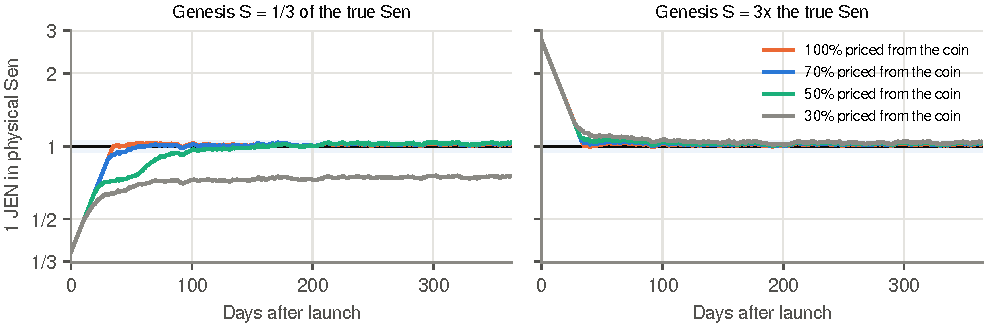
\includegraphics[width=\textwidth]{figs/converge.pdf}
\caption{Convergence of the peg from a wrong genesis weight, by the share of coin-priced value whose price is set from the physical coin. The blue band is $\pm5\%$ (simulated, \texttt{volsim.js}, anchor and band from day 1).}
\label{fig:converge}
\end{figure}

\begin{table}[htbp]
\centering\small
\begin{tabular}{l r r r r}
\toprule
\textbf{Share priced from the physical coin} & \textbf{$S$ starts at $\tfrac13$} & \textbf{$\tfrac12$} & \textbf{$2\times$} & \textbf{$3\times$}\\
\midrule
90--100\% & 34 & 20 & 20 & 34\\
70\% & 46 & 21 & 20 & 57\\
50\% & 98 & 27 & 75 & 84\\
30\% & $>$365 (stuck near 0.75) & 303 & 321 & 321\\
\bottomrule
\end{tabular}
\caption{Days until 1~\JEN{} stays within 5\% of 1~\SEN{} (simulated, \texttt{converge.js}). A 30-day launch phase without anchor and band shortens this to 0--22 days at 70\% or more, but leaves the launch unprotected.}
\label{tab:converge}
\end{table}

The lesson is practical as much as technical: wallets should quote coin prices and coin ratios from metal prices by default, not from the network's $S$. A reading taken from payments can feed on itself once prices are set from it, as the authors of UTXOracle note for their own estimator \cite{utxoracle}.

%=====================================================================
\FloatBarrier
\section{Three currencies, six coins: a self-correcting system}\label{sec:selfcorrect}

Sections~\ref{sec:pom}--\ref{sec:peg} describe the machinery. This section states the thesis behind it: physical money and electronic money each fail in ways the other does not, a single currency is easy to attack, and three linked currencies, each tied to a physical coin, form a system that measures itself, points to where it is being attacked, and pulls itself back. The thesis is stated as a proposal; Section~\ref{sec:sclimits} says where it holds and where it does not.

\subsection{Two kinds of money, complementary failures}

\begin{table}[htbp]
\centering\small
\begin{tabularx}{\textwidth}{l Y Y Y}
\toprule
\textbf{Problem} & \textbf{Physical metal alone} & \textbf{Cryptocurrency alone} & \textbf{Zen (both, linked)}\\
\midrule
Safe storage & needs a vault or trusted custodian; theft & keys on a phone; no vault & savings can sit in either form; neither needs a custodian\\
Long-distance payment & slow, costly, risky to ship & instant & paid electronically; metal stays home\\
Counterfeiting & fake coins, hard to test & impossible (signatures) & counterfeit physical coins show up as a divergence in the readings (Section~\ref{sec:exreading})\\
Volatility & value of the metal only & large swings & electronic coin tracks a fixed metal weight\\
Forks and thousands of coins & -- & value split across chains and copies & one design, three metals, each with a physical anchor that a copy cannot take with it\\
Small daily payments & small coins cost more to mint than they are worth & fees and block space & Jen in sixths of a Sen; channels below that\\
Single point of attack & one metal, one market & one chain, one price & three chains and three cross rates that check each other\\
\bottomrule
\end{tabularx}
\caption{What each kind of money lacks, and how Zen combines them.}
\label{tab:complement}
\end{table}

\subsection{Why three, and not one or two}
With $n$ linked currencies there are $n(n-1)/2$ exchange rates. With \textbf{one} currency there is no rate at all: nothing inside the system can say its value has been pushed. With \textbf{two} there is one rate. If that rate departs from the ratio of the two metals, something is wrong, but the system cannot say which side moved: a push on Jen and a push on Ken in the other direction look identical. With \textbf{three} there are three rates, of which two are independent, and the attacked currency becomes identifiable.

Let $x_i$ be the log deviation of chain $i$'s electronic coin from its physical coin (zero when $1~\JEN=1~\SEN$). Each electronic cross rate, compared with the ratio of the metals in the two physical coins, gives a residual
\begin{equation}
r_{ij} = x_i - x_j \qquad (\text{e.g. } r_{\text{Jen,Ken}} = \log\frac{\text{Jen coins per Ken coin on the exchange}}{\text{Sen per Ten from metal prices}}).
\end{equation}
An attack on Jen moves $r_{\text{Jen,Ken}}$ and $r_{\text{Jen,Yen}}$ together and leaves $r_{\text{Ken,Yen}}$ flat: the odd one out is named. This is the logic of triple modular redundancy and of $2f+1$ fault tolerance with $f=1$: three members can identify one faulty member. Triangular arbitrage keeps the three electronic rates consistent with each other ($\tfrac{J}{K}\cdot\tfrac{K}{Y}\cdot\tfrac{Y}{J}=1$) whatever happens, so the signal is not in the triangle closing; it is in each rate against its metal ratio.

\paragraph{Everything is public, in grams.} The triangle of cross rates is only what an outside observer sees. Inside Zen there is much more, and all of it is public. Each chain publishes its coin weight $S$, the grams of its money that make one coin, in every block. Every trade between the chains settles on-chain, so the gram rate of each pair is public. And coin-priced trades (``1~\KEN{} for 212~\JEN'') carry the coin ratio that traders take from the metal markets. Together these give every chain three readings of what its physical coin is worth (Section~\ref{sec:exreading}): its own coin-priced payments, and one reading through each of its two exchange pairs, built from the partner chain's public weight, the pair's gram rate and the coin ratio:
\begin{equation}
I_{\text{Jen}}^{(\text{Ken})} = S_{\text{Ken}}\times\frac{\text{Ken grams per Jen gram}}{\text{Jen coins per Ken coin}} .
\end{equation}
That is nine public readings, recomputed by every node and every wallet from the blocks and the batch auctions, with no oracle. An attacker can bias six things: the payments of each chain, and the coin-priced orders of each pair. Each leaves its own fingerprint. Fake payments on Jen move one reading, Jen's own, and leave Jen's two exchange readings in agreement against it. Wrong-ratio orders on Jen--Ken move two readings in opposite directions, Jen's reading through Ken and Ken's reading through Jen, while both chains' payments disagree with them. Because every reading is redundant, the smallest set of biased components that explains all nine is the attack, and it is unique for any attack on one or two components.

\begin{figure}[htbp]
\centering
\begin{tikzpicture}[
  ch/.style={box,line width=1.1pt,minimum width=2.6cm,minimum height=1.0cm},
  ph/.style={box,minimum width=1.9cm,minimum height=0.8cm,font=\sffamily\scriptsize}]
  \node[ch,draw=yen] (Y) at (0,3.8) {\textbf{Golden Yen}};
  \node[ch,draw=ken] (K) at (-4.4,0) {\textbf{Silver Ken}};
  \node[ch,draw=jen] (J) at (4.4,0) {\textbf{Bronze Jen}};
  \draw[arr,{Stealth[length=2mm]}-{Stealth[length=2mm]}] (Y) -- node[lbl,above left=2pt and 2pt,pos=0.55] {KEN/YEN\\vs gold/silver} (K);
  \draw[arr,{Stealth[length=2mm]}-{Stealth[length=2mm]}] (Y) -- node[lbl,above right=2pt and 2pt,pos=0.55] {JEN/YEN\\vs gold/copper} (J);
  \draw[arr,{Stealth[length=2mm]}-{Stealth[length=2mm]}] (K) -- node[lbl,below=2pt] {JEN/KEN vs silver/copper} (J);
  \node[ph,fill=yen!12,draw=yen] (R) at (0,5.6) {Ren, 4\,g gold};
  \node[ph,fill=ken!10,draw=ken] (T) at (-4.4,-1.9) {Ten, 3\,g silver};
  \node[ph,fill=jen!10,draw=jen] (Sn) at (4.4,-1.9) {Sen, 2\,g copper};
  \draw[arr,dashed,{Stealth[length=2mm]}-{Stealth[length=2mm]}] (R) -- node[lbl,right=2pt] {coin points, shops} (Y);
  \draw[arr,dashed,{Stealth[length=2mm]}-{Stealth[length=2mm]}] (T) -- node[lbl,left=2pt] {coin points, shops} (K);
  \draw[arr,dashed,{Stealth[length=2mm]}-{Stealth[length=2mm]}] (Sn) -- node[lbl,right=2pt] {coin points, shops} (J);
  \node[box,fill=wash,text width=4.6cm,font=\sffamily\scriptsize] at (0,1.35) {Each chain also reads itself from its own payments (Section~\ref{sec:peg}). Three readings per chain; the median counts.};
\end{tikzpicture}
\caption{Six coins, three cross rates. Each electronic cross rate is checked against the ratio of the metals; each electronic coin is also traded against its own physical coin at coin points and in shops. An attack on one chain bends two sides of the triangle and leaves the third straight.}
\label{fig:triangle}
\end{figure}

\subsection{Reading the signals}
Because every chain has three readings (its own payments and two exchange pairs, Section~\ref{sec:exreading}) and the world has independent markets for the three metals, distinct events leave distinct patterns:

\begin{table}[htbp]
\centering\small
\begin{tabularx}{\textwidth}{Y Y Y}
\toprule
\textbf{Pattern} & \textbf{Likely cause} & \textbf{What corrects it}\\
\midrule
One chain's two cross residuals move together; the third stays flat & attack on that chain's peg & median of three holds $S$; arbitrage and defenders push back\\
One chain's payment reading departs from both of its exchange readings; cross residuals normal & trust in that chain's \emph{physical} coin has changed (counterfeits) & median keeps the electronic coin at metal value; physical testing\\
All three move together against metal prices; cross residuals flat & common shock: demand for Zen as a whole, or a general metal move & nothing to correct; $S$ follows at the anchor's pace\\
Two chains' payment readings each depart from their own exchange readings & payment attack on both chains & each chain's median holds; both are named\\
One pair's two readings move in opposite directions & wrong-ratio orders on that pair (exchange attack) & the attacker's orders are filled by others at a loss\\
All three readings of one chain move together & a real move of that metal, or an attacker holding the chain's payments and both its pairs at once & the anchor follows at 2.9\% a day; world metal prices tell which (Section~\ref{sec:sclimits})\\
\bottomrule
\end{tabularx}
\caption{Signals and their likely causes.}
\label{tab:signals}
\end{table}

\subsection{The correcting forces}
Detection is useful only if something pulls the system back. Four forces do, none of them a central party:
\begin{enumerate}
\item \textbf{The protocol.} Each chain's day value is the median of three readings, and $S$ moves at most 2.9\% a day within a $\pm10\%$ band (Section~\ref{sec:defences}). A pushed reading is outvoted or held.
\item \textbf{Triangular arbitrage.} If the three electronic rates disagree with each other, traders profit by cycling through them until they agree.
\item \textbf{Coin-for-coin arbitrage.} Where an electronic coin buys more or less than its physical coin (at stream nodes that act as coin points, Section~\ref{sec:channels}, or in shops that accept both), traders buy the cheap form and sell the dear one, pulling the two together.
\item \textbf{Defenders.} Because the signal is public and attributes the attack, shops, exchanges and community funds know where to add honest payments; in simulation half the attacker's money undoes the push at about a twentieth of his cost (Section~\ref{sec:defences}).
\end{enumerate}

\subsection{How fast an attack is seen}
A model of the nine readings makes the claim concrete \st{simulated}. Every hour, each chain's payment reading has noise of about 5\% (1\% a day) and each exchange reading about 3\% (0.67\% a day), the same noise as in the three-chain peg model (\texttt{tri2.js}); thin, young markets get three times as much. A detector, which any node or wallet can run on the public data, fits the readings over the last 1 to 24 hours with the smallest set of biased components; it raises an alarm when some set explains the readings much better than none, with the threshold set for about one false alarm in five quiet years. The day after the alarm it names the components. An attacker pushes his readings by 2\% to 25\%; 25\% is roughly what the \$5M attacker of Table~\ref{tab:defences} achieves on Jen's payment reading.

\begin{figure}[htbp]
\centering
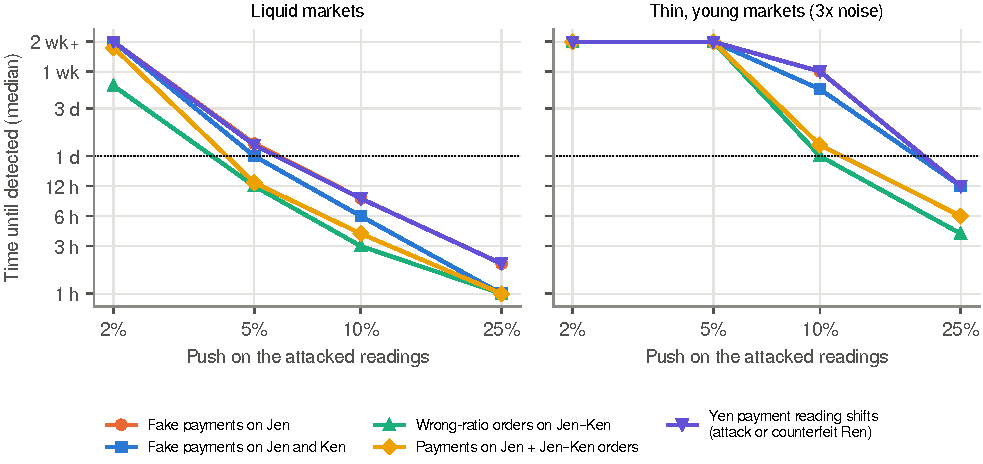
\includegraphics[width=\textwidth]{figs/detect9.pdf}
\caption{Time until an attack is detected from the nine public readings, by attack type and size (median of 400 runs per point; simulated, \texttt{detect9.py}). Fake payments on Jen and a shift of Yen's payment reading behave identically and overlap. ``2 wk+'' means not detected within 14 days.}
\label{fig:detect9}
\end{figure}

\begin{table}[htbp]
\centering\small
\begin{tabularx}{\textwidth}{Y r r r r r r}
\toprule
& \multicolumn{3}{c}{\textbf{Liquid markets}} & \multicolumn{3}{c}{\textbf{Thin markets}}\\
\cmidrule(lr){2-4}\cmidrule(lr){5-7}
\textbf{Attack} & \textbf{5\%} & \textbf{10\%} & \textbf{25\%} & \textbf{5\%} & \textbf{10\%} & \textbf{25\%}\\
\midrule
Fake payments on Jen & 32 h & 9 h & 2 h & -- & 7 d & 12 h\\
Fake payments on Jen and Ken & 24 h & 6 h & 1 h & -- & 5 d & 12 h\\
Wrong-ratio orders on Jen--Ken & 12 h & 3 h & 1 h & -- & 24 h & 4 h\\
Payments on Jen + Jen--Ken orders & 13 h & 4 h & 1 h & -- & 31 h & 6 h\\
Yen payment reading shifts (attack or counterfeit Ren) & 31 h & 9 h & 2 h & -- & 7 d & 12 h\\
\midrule
\textit{Right components named, within a day of the alarm} & 99--100\% & 99--100\% & 99--100\% & -- & 74--100\% & 99--100\%\\
\bottomrule
\end{tabularx}
\caption{Median time to detection from the nine public readings (simulated, \texttt{detect9.py}). ``--'': not detected within 14 days, because a 5\% push in thin markets stays inside normal noise. A 2\% push is not detected in either case; it is within the normal 2--4\% wander of $S$.}
\label{tab:detect9}
\end{table}

Three results stand out. First, an attack of the size that matters is seen within hours: a 25\% push on the readings within one or two hours in liquid markets, and within half a day in thin ones. $S$ changes only when a day's reading closes, and then within the day clip and the anchor's band, so the alarm comes before the attacked day has even been counted. Second, the attack is \emph{named}, not only seen, in 99--100\% of runs once it is above the noise, including attacks on two chains at once and combinations of payments and exchange orders. Third, pushes smaller than the normal wander are not detected, and need not be: they are smaller than the error the peg already tolerates.

Because the chains are public, the alarm also points to the accounts. Payments that count toward $S$ come from accounts with rested balances and bonded receivers (Section~\ref{sec:defences}), so watchers can list which new bonded receivers moved together, where their money came from, and when it arrived. The same data separates an attack from a counterfeit wave: fake payments on Yen come from a few recently bonded accounts with concentrated value, while a loss of trust in physical Ren shifts the prices of many long-established shops at once.

\subsection{One money for the user}
To a user, Zen can look like one currency in three sizes, as gold, silver and copper once were. A wallet holds all three and shows a single balance in the unit its owner chooses (for example Sen, or the local currency at today's metal prices); it pays large amounts in Yen, everyday amounts in Ken or Jen and fractions in Jen over channels, swapping between them through stream nodes in the same atomic payment (Section~\ref{sec:channels}). Unlike historical trimetallism, the ratios between the three are not fixed by law but float with the metal markets, so Gresham's law has no fixed ratio to exploit. The cost of that freedom is that a balance shown in one unit moves when the metal ratios move; the gold--silver ratio, for instance, changes over years.

\subsection{Where the thesis holds and where it does not}\label{sec:sclimits}
\begin{itemize}
\item \textbf{``Instantly detectable''} holds in a practical sense: every node can compute all nine readings from public data every block, and attacks large enough to matter are named within hours. Small pushes take days, or stay hidden inside normal noise, where they do no harm.
\item \textbf{One chain fully held.} An attacker who controls a chain's payments \emph{and} both of its exchange pairs moves all three of its readings together. That looks exactly like a genuine move of that metal. Zen's answer is the anchor, which lets $S$ follow any such move at no more than 2.9\% a day, and the world metal prices, which anyone can compare: if copper did not move, the attack is visible. Holding Jen's payments and two exchange pairs costs on the order of \$60M a month at one million payments a day (Section~\ref{sec:exreading}).
\item \textbf{Common shocks are invisible by design.} If demand for all of Zen rises or falls, or all metals move together, all nine readings stay consistent. That is correct behaviour: there is nothing to correct.
\item \textbf{Correction needs liquidity and honest pricing.} Arbitrage only works where the exchange and coin points have volume, detection in thin markets takes days instead of hours, and the peg converges only if most coin-priced shops price from the metal (Section~\ref{sec:converge}). Before Ken and Yen exist, Jen has its payments and its coin-for-coin market only.
\item \textbf{Metal prices enter through people.} No metal price is in consensus. The metal ratios enter the readings through the coin ratios traders quote, and through the shops that price in coins; watchers can compare everything with world metal prices, but the chains do not.
\end{itemize}
